\chapter{In-Train Forces: Draft Gear, Traction, and the International Benchmark}
\label{ch:benchmark}
\chaptermark{In-Train Forces and the Benchmark}

% ---------------------------------------------------------------------------
% Part II, tier 3 of the plan in Ch. 10. Sources: SIMULATOR_VALIDATION_NOTE.md
% (log 2026-09-26 to 2026-10-04), simulator2/draft_gear.py,
% simulator2/ltd_benchmark.py, simulator2/torch_rhs.py (_notch_force,
% _db_at_notch), the benchmark write-up of 2026-10-04.
% Numbers regenerate with:
%   python scripts/compare_ltd_benchmark.py --tag _s3k \
%       --json results/ltd_benchmark/compare_s3k.json
%   python scripts/compare_ltd_benchmark.py --tag _s3k_tau1 \
%       --json results/ltd_benchmark/compare_s3k_tau1.json
%   python paper/scripts/plot_ltd_benchmark.py
% ---------------------------------------------------------------------------

\Cref{ch:critique} found that the legacy simulator solves its equations correctly but that nothing yet shows those equations describe a freight train. This chapter supplies the first external evidence. It reproduces the international benchmark of longitudinal train dynamics simulators \cite{Spiryagin2017BenchmarkQuestions}, whose four freight trains were run by nine established simulators and published together \cite{Wu2018BenchmarkResults}, and asks whether this simulator lands within their spread.

The benchmark could not be run on the legacy model. It specifies a friction draft gear, notch-controlled traction and a dynamic brake, none of which the legacy simulator had, and it uses drawbars and resistance and curving laws of its own. Building those models is half of this chapter, and the draft gear, which is finding F3 of \cref{tab:critique_findings}, is the larger part. The benchmark then tests them. Taking part therefore corrects two findings and validates the in-train force model in a single step.

\section{The benchmark}
\label{sec:bench_spec}

Longitudinal dynamics simulators have mostly grown up as in-house tools, each with its own numerical methods and assumptions, and until recently there was no common basis on which to compare them (\cref{ch:related}). The benchmark of \cite{Spiryagin2017BenchmarkQuestions} provides one. It is fully self-contained: the trains, the track, the driving commands and the force laws are all printed, and participants build their own models from them.

\subsection{Trains, track and driving}

The benchmark defines four freight trains, each driven for 5,000\,s (\cref{tab:bench_trains}). Locomotives are of two types, 134\,t and 195\,t, both on six axles; wagons are 128\,t or 160\,t on four axles. Wagons run in pairs joined by a slackless drawbar, and every other connection is a coupler with 10\,mm of total slack and a friction draft gear at each end. Trains 2 and 4 use distributed power: remote locomotives receive the lead locomotive's notch 3\,s later.

\begin{table}[htbp]
    \centering
    \small
    \begin{tabular}{c>{\raggedright}p{7.2cm}rr}
        \toprule
        Train & Consist & Mass (t) & Length (m) \\
        \midrule
        1 & 2 locomotives (type 1) + 50 wagons & 6,668 & 796 \\
        2 & Train 1 twice, distributed power & 13,336 & 1,592 \\
        3 & 3 locomotives (type 2) + 240 wagons & 38,985 & 2,713 \\
        4 & 2 locomotives + 120 wagons + 1 locomotive + 120 wagons (all type 2) & 38,985 & 2,713 \\
        \bottomrule
    \end{tabular}
    \caption{The four benchmark trains \cite{Spiryagin2017BenchmarkQuestions}. A published corrigendum changes the middle locomotive of Train 4 to type 2; the paper's stated mass and length already correspond to that consist.}
    \label{tab:bench_trains}
\end{table}

The track is 50\,km of tabulated gradients with curves of 300\,m radius, each entered and left through 50\,m transitions. The driving commands are notch sequences in time for each train, written to keep it within 110\% of a speed board. The paper asks for the lead locomotive's position and speed, the force and draft-gear deflection at selected connections, and the maximum tension and compression at every connection, all at 10\,ms.

\subsection{What the benchmark leaves out}

Air brakes are excluded on purpose. Traction and dynamic braking alone control the trains, so the benchmark tests couplers, traction, dynamic braking, resistance and grade, which is to say the in-train force problem, but not the brake pipe. Findings F1 and F2 of \cref{ch:critique} are therefore outside its reach and are taken up separately in \cref{ch:v3_sim}.

The paper also leaves several choices to participants: the form of the draft gear model, which is given only as a drop-hammer test curve; the rate at which the notch may change; and whether to model starting resistance. Each choice made here is stated where it is made.

\subsection{The participants}

Nine simulators took part: TABLDSS, UM, CRE-LTS, TDEAS, PoliTo, TsDyn, CARS, BODYSIM and VOCO \cite{Wu2018BenchmarkResults}. The results paper finds basic agreement on locomotive, resistance and grade forces, with the largest differences in the draft gear models. Six of the simulators, TABLDSS, UM, CRE-LTS, TDEAS, TsDyn and CARS, are in general agreement on in-train forces; PoliTo and BODYSIM showed draft-gear instabilities, and VOCO ran Train 1 only. This chapter calls the six the \emph{core} group and treats landing inside their range as the test.

\section{A friction draft gear}
\label{sec:bench_draft_gear}

\subsection{What the benchmark specifies}

A benchmark connection is the coupler slack plus two draft gears in series, one in each vehicle's end. Each gear is specified only by its drop-hammer test: a plot of force against deflection on loading and on unloading (\cref{fig:bench_draft_gear}). The gear travels about 82\,mm and reaches about 2.1\,MN at full travel on loading. On unloading it follows a much lower curve, and the area between the two is the energy the gear dissipates through friction in one cycle. The curves were digitized from the paper's figure by pixel colour, giving a peak of 2,126\,kN at 82.4\,mm, and checked against the original by overlay.

\begin{figure}[htbp]
    \centering
    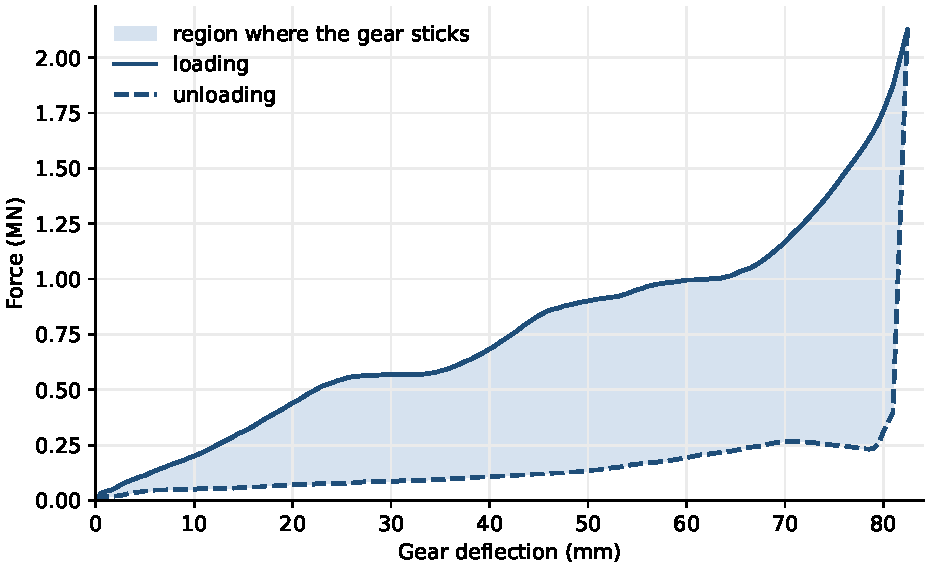
\includegraphics[width=0.72\textwidth]{figures/draft_gear_envelope.pdf}
    \caption{Loading and unloading curves of one benchmark draft gear, digitized from the drop-hammer plot of \cite{Spiryagin2017BenchmarkQuestions}. Between the two curves the stateful model of \cref{sec:bench_gear_stateful} holds the gear stuck.}
    \label{fig:bench_draft_gear}
\end{figure}

With equal gears in series, each carries the connection force and takes half the travel. Once the 10\,mm slack is closed, the deflection $g$ of each gear is half the remaining connection extension. The gear closes in both draft and buff, so the characteristic is odd in the connection extension, and beyond full travel the gear is solid and a stiff end stop, $k_{\mathrm{lock}} = 5\times10^{8}$\,N/m, takes over. Drawbars have no slack and use the same gears.

\subsection{A first model, and why it failed}

The simplest way to turn two curves into a force law is to switch between them on the sign of the closing velocity, smoothed so that the force stays continuous:
\begin{equation}
    F = F_U(g) + \bigl(F_L(g) - F_U(g)\bigr)\,\frac{1 + \tanh\!\bigl(\mathrm{sgn}(e)\,\dot e / v_t\bigr)}{2},
    \label{eq:bench_velocity_switch}
\end{equation}
where $F_L$ and $F_U$ are the loading and unloading curves, $e$ is the connection extension, and $v_t$ is a small transition velocity. This stateless form is used in the literature. % TODO: cite the source of the velocity-switch draft gear (Wu et al. 2014, VSD 52(6)).
It proved unusable at the production step. The slope of the switch, $(F_L - F_U)/2v_t$, acts as a damper of about $4\times10^{7}$\,N\,s/m at $v_t = 5$\,mm/s, some eighty times the legacy coupler's damper and far outside the stability region of explicit fourth-order Runge--Kutta at 0.02\,s. \Cref{tab:bench_switch_energy} shows the consequence on the realistic 10-car consist of \cref{sec:critique_convergence}.

\begin{table}[htbp]
    \centering
    \small
    \begin{tabular}{cccc}
        \toprule
        $v_t$ (m/s) & $\Delta t = 0.02$\,s & $\Delta t = 0.005$\,s & Converged dissipation \\
        \midrule
        0.005 & 333\,kJ (residual $4.7\times10^{-3}$) & 28\,kJ & 11\,kJ \\
        0.02  & 100\,kJ (residual $1.4\times10^{-3}$) & 6.2\,kJ & 6.2\,kJ \\
        0.1   & 4.3\,kJ & 4.3\,kJ & 4.3\,kJ \\
        \bottomrule
    \end{tabular}
    \caption{Energy dissipated in the couplers over 30\,s by the velocity-switch gear of \cref{eq:bench_velocity_switch}, on a realistic 10-car consist, with the energy-audit residual where it is not at its floor of $1.6\times10^{-8}$.}
    \label{tab:bench_switch_energy}
\end{table}

At the production step the switch manufactured about thirty times the true dissipation. And even with the integration converged, the dissipation depends on $v_t$, a parameter with no physical meaning: a friction gear held still does not slide back to its unloading curve, but this model does whenever the closing velocity is zero. The model was kept for the record and not used.

\subsection{The stateful model}
\label{sec:bench_gear_stateful}

The model used instead gives each connection a state of its own, the gear force $z$. While $z$ lies between the two curves the gear sticks, and its force changes elastically with the connection extension,
\begin{equation}
    \dot z = k_t\,\dot e,
    \qquad
    F_U(g) \le |z| \le F_L(g),
    \label{eq:bench_gear_stateful}
\end{equation}
where $k_t$ is a transitional stiffness. When $z$ reaches either curve the gear slides along it, which in the implementation is the clamp on the right of \cref{eq:bench_gear_stateful}. The connection force is $z$. A gear held still keeps its force, as a friction gear does, and because both curves start at zero there is no force jump when the slack closes. The state vector of an $N$-vehicle train grows from $4N$ entries to $4N + (N - 1)$.

The model was checked as the legacy force laws were in \cref{sec:critique_verification}. Its energy audit closes to $1.6\times10^{-8}$ at the production step, the same floor as at fine steps, and the coupler dissipation at the production step is within 0.4\% of its converged value, against a factor of thirty for the velocity switch. Thirteen tests check its behaviour: it follows the loading curve out and the elastic line and unloading curve back; it holds its force at rest; small reversals inside the envelope are elastic, with no net work; the force never leaves the envelope; momentum is exact; and it is stable on 26\,t empty wagons at 0.02\,s.

The one modelling choice is $k_t$. The drop-hammer plot's near-vertical unloading drop implies about $7\times10^{8}$\,N/m per connection. A smaller value rounds off the corner of the loop where loading turns to unloading, and captures less of its area (\cref{tab:bench_kt}).

\begin{table}[htbp]
    \centering
    \small
    \begin{tabular}{ccc}
        \toprule
        $k_t$ (N/m) & Loop area captured, 25\% travel & Full travel \\
        \midrule
        $1\times10^{8}$ & 90\% & 86\% \\
        $3\times10^{8}$ & 97\% & 97\% \\
        $7\times10^{8}$ & 99\% & 100\% \\
        \bottomrule
    \end{tabular}
    \caption{Share of the drop-hammer hysteresis loop captured by the stateful gear against the transitional stiffness $k_t$.}
    \label{tab:bench_kt}
\end{table}

The value $10^{8}$\,N/m keeps fourth-order Runge--Kutta stable at 0.02\,s on empty 26\,t wagons, at the cost of 10--14\% of the loop's dissipation. The benchmark trains are all loaded, 128 to 195\,t per vehicle, and ask for output every 10\,ms, so they are run with the drop-hammer value $7\times10^{8}$\,N/m at $\Delta t = 0.01$\,s. \Cref{sec:bench_step} shows that the choice changes the benchmark results by under 1\%.

\subsection{Convergence, a wrong prediction}

The stateful gear was expected to converge better than the legacy coupler, since it removes the force jump at the slack edge that \cref{sec:critique_convergence} identified as the cause of non-convergence. That prediction was wrong (\cref{tab:bench_gear_convergence}).

\begin{table}[htbp]
    \centering
    \begin{tabular}{ccccc}
        \toprule
        $\Delta t$ (s) & Max $|\Delta v|$ (m/s) & 99th pct. & Median & Final $|\Delta x|$ (m) \\
        \midrule
        0.02   & $2.5\times10^{-2}$ & $5.2\times10^{-3}$ & $9.6\times10^{-5}$ & $1.6\times10^{-4}$ \\
        0.01   & $2.8\times10^{-2}$ & $4.7\times10^{-3}$ & $9.2\times10^{-5}$ & $1.3\times10^{-4}$ \\
        0.005  & $8.8\times10^{-3}$ & $2.0\times10^{-3}$ & $3.7\times10^{-5}$ & $4.1\times10^{-5}$ \\
        0.0025 & $9.5\times10^{-3}$ & $1.8\times10^{-3}$ & $3.2\times10^{-5}$ & $5.7\times10^{-5}$ \\
        \bottomrule
    \end{tabular}
    \caption{Velocity and position error of the simulator with the stateful draft gear on the realistic 10-car consist, against a reference at $\Delta t = 0.000625$\,s. Compare \cref{tab:critique_convergence} for the legacy coupler.}
    \label{tab:bench_gear_convergence}
\end{table}

The median error at the production step is about a hundred times that of the legacy coupler, and the reference itself agrees with a run at half its step only to $4.4\times10^{-3}$\,m/s. The reason is that the gear's rate switches between sticking and sliding, and the slopes of the digitized curves change at every table point, every 0.5\,mm. While couplers are in contact the right-hand side is discontinuous almost everywhere, and trajectories converge at first order at best. Energy closes and dissipation converges; trajectories do not converge at the rate of the method. The published simulators use small steps for friction gear for this reason. Whether the remaining error matters is a question the benchmark can answer directly, by asking whether it shows up at the level at which the nine simulators agree.

\subsection{What the gear means for the surrogate}

The legacy coupler's force is a function of the current stretch and its rate, which is why GNS-1 can compute it as an edge feature (\cref{sec:arch_network}). The friction gear's force depends on its loading history. Once the corpus is generated with it, a surrogate edge must carry the gear state, or infer it, and the coupler becomes a harder learning problem than the one \cref{ch:training} solved. \Cref{ch:surrogate_revised} takes this up.

\section{Traction, dynamic braking and the remaining laws}
\label{sec:bench_traction}

\subsection{Notch traction}

Benchmark locomotives are diesel-electric units controlled by eight traction notches. At notch $n$ the tractive force is a fraction of the maximum tractive effort until the power available at that notch is reached, and power-limited above it:
\begin{equation}
    F(n, v) =
    \begin{cases}
        \dfrac{n}{8}\,T_{\max} & \text{if } \dfrac{n}{8}\,T_{\max}\,v < \left(\dfrac{n}{8}\right)^{2} P_{\max}, \\[2ex]
        \left(\dfrac{n}{8}\right)^{2} \dfrac{P_{\max}}{v} & \text{otherwise.}
    \end{cases}
    \label{eq:bench_notch}
\end{equation}
This has the same structure as the legacy law of \cref{eq:ltd_power_cap}, a force limit and a power limit, so what was needed was the mapping from notch to force and power, for each locomotive type. The benchmark leaves the rate at which the notch may change to participants. Here the notch passes through a first-order lag with the simulator's existing traction time constant of 5\,s, and while the lag carries it between integer notches the force is blended linearly between the two neighbouring notch curves, so that it stays continuous.

\subsection{Dynamic brake}

The dynamic brake, absent from the legacy model (F5), is a new force channel with eight notches of its own. Each notch's braking force rises with speed to a plateau and is capped by the braking power at high speed. The paper's table of these curves is internally inconsistent as printed for notches 1 to 6, so it was read against the paper's own plotted curves: every notch rises on a common ramp to a plateau of $\mathrm{DB}_{\max}\,n/8.7$ for notches 1 to 3 and $\mathrm{DB}_{\max}\,n/7.5$ for notches 4 to 6, under the power cap. That reading reproduces the crossover speeds visible in the plotted curves. A signed command carries both channels: positive values are traction notches, negative values dynamic-brake notches.

\subsection{Resistance, curving, grade and drawbars}

The benchmark's running resistance is given per vehicle as
\begin{equation}
    R = Q\,m\left(2.943 + \frac{89.2}{m_a} + 0.0306\,V + \frac{0.122\,V^{2}}{m}\right)\ \text{N},
    \label{eq:bench_resistance}
\end{equation}
with $m$ the vehicle mass and $m_a$ the axle load in tonnes, $V$ the speed in km/h, and $Q = 3.2$ for the lead locomotive and 1 for every other vehicle. It has the Davis form of \cref{eq:ltd_davis} and converts exactly into per-vehicle coefficients $A$, $B$ and $C$, so no change to the simulator's resistance law was needed. Curving resistance is 6,116$/R$ newtons per tonne; the simulator's linear law of \cref{eq:ltd_curvature} reproduces it exactly with $c_\kappa = 0.8925$. The paper's gradient table is read as steps, which integrates to the elevation profile it plots: a 93.6\,m valley, a 145.1\,m summit and 113.3\,m at 50\,km. Interpolating the gradients linearly instead ends about 5\,m high. Drawbars are connections with zero slack.

\section{Running the benchmark}
\label{sec:bench_run}

The trains, track, controls and laws above are encoded as a scenario set for the GPU integrator of \cref{ch:gpu_dataset}, with the paper's tables transcribed from its PDF by script rather than by hand. All four trains run as one batch with the stateful gear at $k_t = 7\times10^{8}$\,N/m, fourth-order Runge--Kutta at $\Delta t = 0.01$\,s, output every 10\,ms, a 5\,s notch lag, and no starting resistance, as the paper allows. Simulating 5,000\,s of all four trains takes about 21 minutes on one RTX~4090, faster than real time. Forty tests cover the harness, and the simulator's existing suite passes unchanged, since every new model is selected explicitly and the legacy path is untouched.

\subsection{A misread starting point}

The first full run put Trains 1 and 2 at 140\% and 116\% of the speed board near 5\,km, well beyond the 110\% the controls were written to allow. Either the light trains accelerated faster here than in the reference simulators, or the harness was playing the controls on the wrong stretch of track, and without the participants' results there was no way to tell.

The results paper settled it. All trains start at the 3\,km location, and only 3 to 50\,km is compared \cite{Wu2018BenchmarkResults}. The questions paper never says so, and the harness had started the lead locomotive at 0\,m, so every notch change was played 3\,km early. With the start moved, the overspeed disappears and the average speeds fall into the participants' range (\cref{tab:bench_start}). One consequence of the correct start is worth stating: the track behind 3\,km falls, and with neither air brakes nor starting resistance the train begins to roll before its first notch.

\begin{table}[htbp]
    \centering
    \small
    \begin{tabular}{lccc}
        \toprule
        Average speed, 3--50\,km (km/h) & Start at 0\,m & Start at 3\,km & Core six \\
        \midrule
        Train 1 & 72.1 & 65.3 & 65.0--65.7 \\
        Train 2 & 70.9 & 64.0 & 63.6--64.4 \\
        Train 3 & 48.7 & 43.9 & 44.0--44.2 \\
        Train 4 & 48.9 & 44.4 & 44.5--44.8 \\
        \bottomrule
    \end{tabular}
    \caption{Average speed with the train started at 0\,m, as first run, and at 3\,km, as the results paper specifies.}
    \label{tab:bench_start}
\end{table}

\section{Results}
\label{sec:bench_results}

\subsection{Speed}

Speed matches on every train. Maximum speed over 3 to 50\,km falls inside the core range for all four trains, and average speed falls inside it for Trains 1 and 2 and 0.1\,km/h below it for Trains 3 and 4. The results paper prints one participant's speed trace for each train; against it, speed differs by 0.4 to 0.6\,km/h root-mean-square, about the resolution of the digitized figure (\cref{fig:bench_speed}). Traction, dynamic braking, resistance, curving and grade are therefore implemented consistently with the established simulators.

\begin{figure}[htbp]
    \centering
    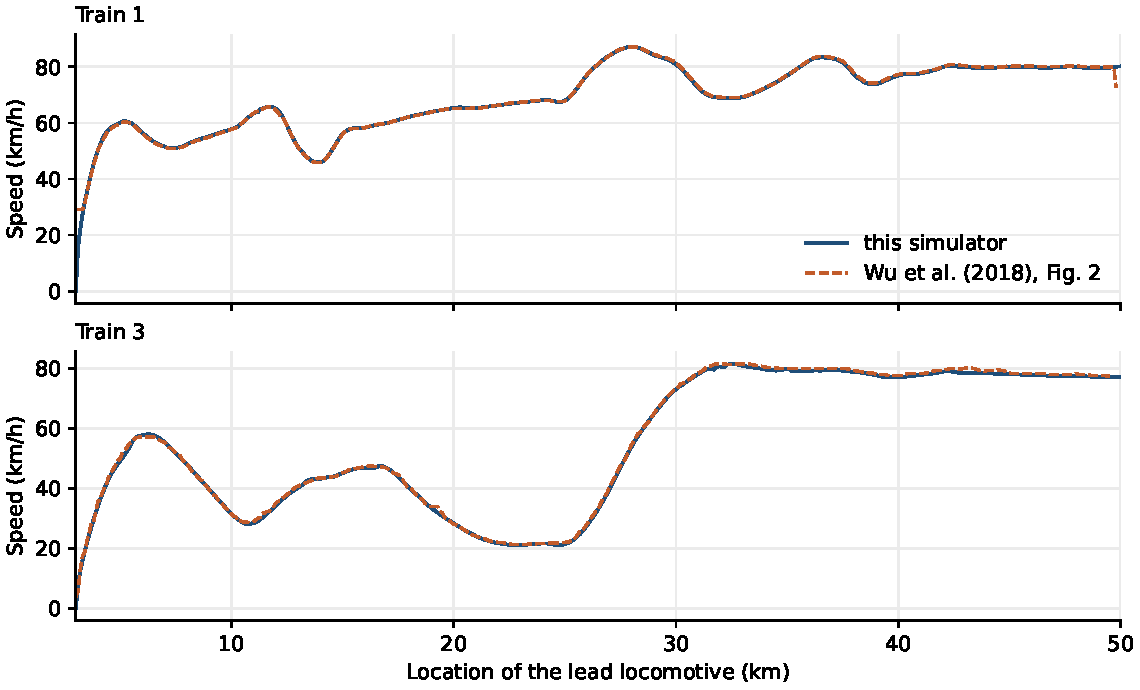
\includegraphics[width=\textwidth]{figures/ltd_benchmark_speed.pdf}
    \caption{Lead locomotive speed against location for Trains 1 and 3, this simulator against the trace printed by \cite{Wu2018BenchmarkResults} (one unnamed participant; Trains 3 and 4 share one trace in the paper).}
    \label{fig:bench_speed}
\end{figure}

\subsection{In-train forces}

\Cref{tab:bench_results} and \cref{fig:bench_strip} compare the 32 force, deflection and speed quantities the results paper tabulates. Twenty-three fall inside the range of the core six, and six more miss it by 2\% or less. The largest tension and compression occur at the same connections the participants report: position 2 on Train 1, 54 on Train 2, 3 on Train 3, and 123 and 122 on Train 4. The long heavy trains, 3 and 4, match best, with every force quantity inside the core range or within 1\% of it.

\begin{table}[p]
    \centering
    \footnotesize
    \setlength{\tabcolsep}{3.5pt}
    \begin{tabular}{clrrrl}
        \toprule
        Train & Quantity & This simulator & Core six & All nine & Against core six \\
        \midrule
        1 & Max speed (km/h)               & 87.1  & 85.0--88.2   & 85.0--88.2   & inside \\
          & Average speed (km/h)           & 65.3  & 65.0--65.7   & 63.9--65.7   & inside \\
          & Largest tension (kN)           & 486   & 549--611     & 549--734     & \textbf{below, 11\%} \\
          & Largest compression (kN)       & 338   & 339--355     & 144--443     & below, 0.4\% \\
          & Mean of max tension (kN)       & 307   & 334--376     & 334--482     & \textbf{below, 8\%} \\
          & Mean of max compression (kN)   & 196   & 195--251     & 79--251      & inside \\
          & Max deflection, tension (mm)   & 52.2  & 15.7--61.0   & 15.7--61.0   & inside \\
          & Max deflection, compression (mm) & 38.0 & 11.8--37.2  & 9.6--48.7    & above, 2.3\% \\
        \midrule
        2 & Max speed (km/h)               & 89.2  & 86.1--90.6   & 86.1--90.6   & inside \\
          & Average speed (km/h)           & 64.0  & 63.6--64.4   & 63.2--64.4   & inside \\
          & Largest tension (kN)           & 730   & 675--1004    & 675--1302    & inside \\
          & Largest compression (kN)       & 407   & 392--580     & 392--580     & inside \\
          & Mean of max tension (kN)       & 418   & 421--631     & 421--631     & below, 0.8\% \\
          & Mean of max compression (kN)   & 262   & 231--348     & 231--348     & inside \\
          & Max deflection, tension (mm)   & 78.1  & 17.1--82.0   & 17.1--92.7   & inside \\
          & Max deflection, compression (mm) & 34.2 & 7.6--38.7   & 7.6--49.3    & inside \\
        \midrule
        3 & Max speed (km/h)               & 81.6  & 80.5--82.1   & 80.5--82.1   & inside \\
          & Average speed (km/h)           & 43.9  & 44.0--44.2   & 43.9--44.2   & below, 0.2\% \\
          & Largest tension (kN)           & 1,639 & 1,625--1,802 & 1,625--2,114 & inside \\
          & Largest compression (kN)       & 977   & 800--1,090   & 624--2,114   & inside \\
          & Mean of max tension (kN)       & 1,172 & 1,157--1,200 & 1,157--1,654 & inside \\
          & Mean of max compression (kN)   & 620   & 486--710     & 395--710     & inside \\
          & Max deflection, tension (mm)   & 149.3 & 30.5--148.6  & 30.5--302.5  & above, 0.5\% \\
          & Max deflection, compression (mm) & 123.2 & 21.2--124.3 & 21.2--195.4 & inside \\
        \midrule
        4 & Max speed (km/h)               & 81.6  & 80.6--82.3   & 80.6--82.3   & inside \\
          & Average speed (km/h)           & 44.4  & 44.5--44.8   & 44.5--44.8   & below, 0.2\% \\
          & Largest tension (kN)           & 1,319 & 1,297--1,411 & 1,297--2,114 & inside \\
          & Largest compression (kN)       & 857   & 722--906     & 722--2,114   & inside \\
          & Mean of max tension (kN)       & 938   & 945--983     & 934--1,765   & below, 0.8\% \\
          & Mean of max compression (kN)   & 507   & 407--547     & 407--819     & inside \\
          & Max deflection, tension (mm)   & 139.8 & 28.8--143.1  & 28.8--227.7  & inside \\
          & Max deflection, compression (mm) & 78.9 & 14.4--89.8  & 14.4--89.8   & inside \\
        \bottomrule
    \end{tabular}
    \caption{This simulator against the nine simulators of \cite{Wu2018BenchmarkResults}, Tables 3--6, with a 5\,s notch lag. Speeds are over 3--50\,km. Deflections are at one connection per train (positions 10, 61, 147 and 146) and are read as the whole connection, both gears and the slack.}
    \label{tab:bench_results}
\end{table}

\begin{figure}[htbp]
    \centering
    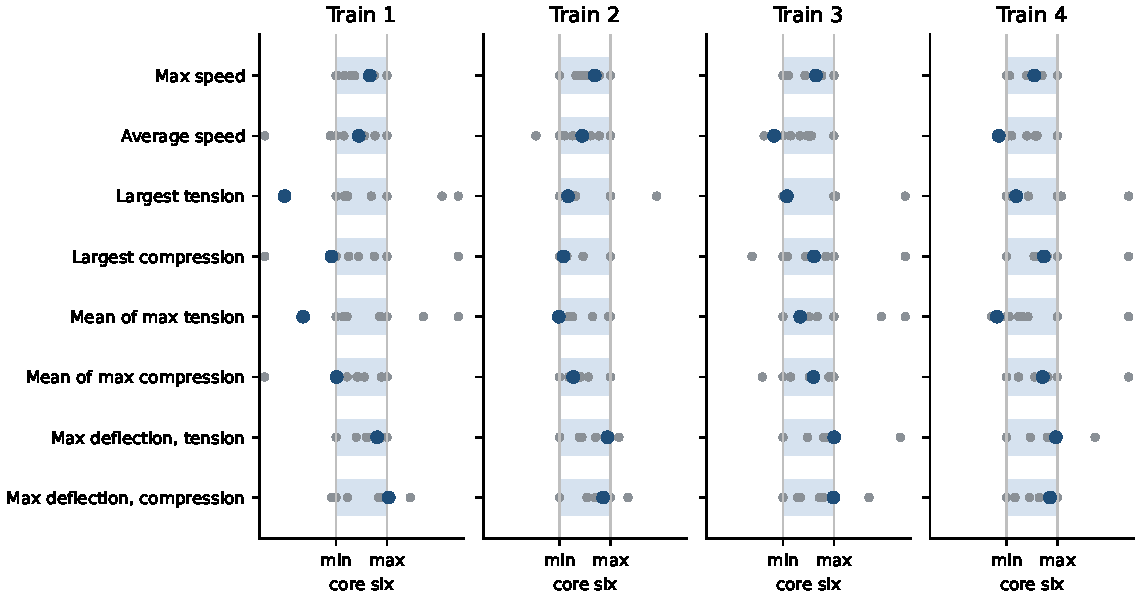
\includegraphics[width=\textwidth]{figures/ltd_benchmark_strip.pdf}
    \caption{The quantities of \cref{tab:bench_results}, each row scaled so that the core six span the shaded band from its minimum to its maximum. Grey dots are the nine participants and the blue dot is this simulator; points far outside the band are drawn at the edge of the panel.}
    \label{fig:bench_strip}
\end{figure}

\subsection{The misses, and the notch lag}

Two quantities miss by more than 2\%, and both are on Train 1. Its largest tension is 486\,kN, where all nine participants report 549 to 734\,kN, 11\% below the lowest. Its mean of maximum tension along the train is 307\,kN against 334 to 376\,kN for the core six, 8\% below.

The peak tension on Train 1 occurs at start-up, 41\,s into the run at about 10\,km/h, when the locomotives first take up the slack of a 52-vehicle train. How hard they do so depends on how fast the notch is allowed to rise, which is exactly the choice the benchmark leaves open. \Cref{tab:bench_notch_lag} varies it.

\begin{table}[htbp]
    \centering
    \small
    \begin{tabular}{lcccc}
        \toprule
        Notch lag & 5\,s (headline) & 2\,s & 1\,s & 0.2\,s \\
        \midrule
        Train 1, largest tension (kN) & 486 & 541 & 565 & 622 \\
        \bottomrule
    \end{tabular}
    \caption{Train 1's largest tension against the notch lag. The core six report 549--611\,kN and all nine 549--734\,kN.}
    \label{tab:bench_notch_lag}
\end{table}

With a 1\,s lag the largest tension on Train 1 rises to 565\,kN and its mean maximum tension to 358\,kN, both inside the core range, and a full re-run of all four trains puts 28 of the 32 quantities inside the core range, with the remaining four within 4\%. The 5\,s lag is kept as the headline anyway. It was chosen before the participants' results were available, and switching to whichever value matches best would be tuning to the answer. The defensible statement is that peak start-up force depends on the unspecified notch rate by up to about 30\%, a span similar to that of the participants themselves, 549 to 734\,kN.

\subsection{Deflections}

Deflection is the weakest comparison. The paper does not define it, and the participants differ by up to five times on the same connection: at position 147 of Train 3, from 31 to 149\,mm within the core six. Several participants report more than one gear's 82.5\,mm of travel, so deflection is read here as that of the whole connection, both gears and the slack. On that reading this simulator sits with TABLDSS, UM, TsDyn and CARS.

\section{Step size, and the production configuration}
\label{sec:bench_step}

The benchmark run uses $\Delta t = 0.01$\,s and $k_t = 7\times10^{8}$\,N/m, while a corpus would be generated at the production step with the softer $k_t = 10^{8}$\,N/m that empty wagons need. Given the convergence of \cref{tab:bench_gear_convergence}, both choices need checking. Trains 1 and 3 were re-run against a reference at $\Delta t = 0.005$\,s with the same $k_t$ (\cref{tab:bench_step}).

\begin{table}[htbp]
    \centering
    \small
    \begin{tabular}{lcc}
        \toprule
        Run & Train 1 & Train 3 \\
        \midrule
        $\Delta t = 0.01$\,s, $k_t = 7\times10^{8}$ (the benchmark run) & 0.1\% & 0.3\% \\
        $\Delta t = 0.02$\,s, $k_t = 10^{8}$ (production) & 0.0\% & 0.6\% \\
        $\Delta t = 0.02$\,s, $k_t = 7\times10^{8}$ & \textbf{+9 to +43\%} & 1.0\% \\
        $k_t = 10^{8}$ against $7\times10^{8}$, both at $\Delta t = 0.005$\,s & 0.1\% & 0.6\% \\
        \bottomrule
    \end{tabular}
    \caption{Largest change in any quantity of \cref{tab:bench_results}, against a reference at $\Delta t = 0.005$\,s with the same transitional stiffness. The last row compares the two stiffnesses directly.}
    \label{tab:bench_step}
\end{table}

Three conclusions follow. The benchmark run at 0.01\,s is converged in every reported quantity, so the comparison stands. The production configuration reproduces the benchmark numbers: $k_t = 10^{8}$\,N/m at 0.02\,s matches the fine-step reference to 0.6\%, and changing $k_t$ moves the reported quantities by under 1\%, so the 10--14\% of loop dissipation it gives up (\cref{tab:bench_kt}) does not appear in these outputs. And the drop-hammer stiffness must never be paired with the production step. At $k_t = 7\times10^{8}$\,N/m and 0.02\,s, Train 1's light wagons fall into a bounded stick-slip oscillation: a steady force of $-317$\,kN reads anywhere from $-277$ to $-450$\,kN, and the root-mean-square second difference of the force is 65\,kN against 0.7\,kN at 0.01\,s. The run completes without error, so only a convergence check exposes it.

Speed and position are insensitive to the step everywhere, within 0.4\,km/h and 2\,m. Instantaneous forces still differ at single moments of impact, by a few kilonewtons at the 99th percentile and up to about 500\,kN at one instant on Train 3. Peak forces over a run are robust; the exact timing of an impact is not, which is the same behaviour \cref{sec:critique_convergence} found for the legacy coupler.

\section{What the benchmark shows}
\label{sec:bench_scope}

The benchmark is a code-to-code validation of the in-train force model. With the benchmark's inputs, this simulator's integrator, traction and dynamic-brake laws, resistance, curving, grade and friction draft gear produce results inside the spread of six established simulators on nearly every reported quantity, and its one real miss is explained by a parameter the benchmark leaves open. That is the external evidence \cref{ch:critique} found missing.

Its limits need stating as clearly.

\begin{itemize}
    \item \textbf{It validates a configuration, not the Part~I corpus.} The configuration that passed uses the friction draft gear, notch traction, the dynamic brake and the benchmark's parameters. \texttt{data/v2} was generated with the legacy Kelvin--Voigt coupler, illustrative parameters and no dynamic brake. The benchmark result transfers to a corpus only if the corpus is regenerated on the validated configuration, which is what Part~III does.
    \item \textbf{It does not test air brakes.} Findings F1 and F2 remain open, and they bear directly on the coupler-force constraint. \Cref{ch:v3_sim} calibrates the brake model against measured data instead.
    \item \textbf{The speed trace is one participant.} The paper's speed figure shows a single unnamed simulator. The tables show all participants' maximum speeds within a few kilometres per hour of each other, so the comparison holds, but it is not against a consensus trace.
    \item \textbf{It is not field data.} Agreement with established simulators bounds this simulator's in-train forces by theirs. It says nothing about how close any of them are to a real train, which would need measurements the benchmark does not provide.
\end{itemize}

Against the findings of \cref{tab:critique_findings}, the chapter closes F3: the coupler now has a friction draft gear, and that gear has been tested against the published simulators. It closes F5 in form, with notch traction and a dynamic brake, while the locomotive parameters for the thesis's own consists remain to be sourced in \cref{ch:v3_sim}. And it checks the form of the resistance law used for F4.

\section{Chapter summary}

To take part in the international benchmark of longitudinal dynamics simulators, the simulator gained a friction draft gear, notch traction, a dynamic brake and drawbars. The draft gear was built twice. A stateless velocity switch manufactured thirty times the true dissipation at the production step and was rejected; a stateful model, in which each connection carries its gear force and sticks between the loading and unloading curves, closes its energy budget at the production step. It converges worse than the legacy coupler, and that was checked rather than assumed.

Run on the four benchmark trains, the simulator matches the participants on speed to within the resolution of the published trace, and lands inside the range of the six core simulators on 23 of 32 force, deflection and speed quantities, with six more within 2\%. The two real misses are on Train 1 at start-up and depend on the notch rate the benchmark leaves open; with a faster notch, 28 of 32 fall inside. The production configuration reproduces the benchmark numbers to under 1\%, provided the soft gear stiffness is used at the production step. The benchmark validates the in-train force model, but not the air brake and not the Part~I corpus, which used none of these models. The next chapter takes up the air brake and the remaining findings, and assembles the corrected simulator.
